\begin{center}{\large\bf 5. Analysis \& Results}\end{center}

\leftline{{\bf5.1 \ Clone Fragment Experiment}}

%Clone fragments refer to code in software. During its life (as a clone), fragment may undergo modification by developers, especially during software maintenance. 
In order to consider changes in clone fragments, we consider three metrics of clone fragments (with respect to the software version in which they were detected): {\em life, ischanged and change time}. These will help us understand how a clone changes in its life (as a clone). 
{
\tabcolsep=2.5pt 
\scriptsize
\begin{center}
\begin{tabular}{c}
{\bf Table 2.\ Clone Fragment  Change Statistic of ArgoUML}\\ 
\end{tabular}
\begin{tabular}{|c|c|c|c|c|}
\hline
Change Times&0&1&2&3\\ \hline
Number&24327&982&109&4\\ \hline
Total&24327&\multicolumn{3}{c}{ 1095}\vline \\
 \hline
\end{tabular}
\end{center}
}
{
\tabcolsep=2.5pt 
\scriptsize
\begin{center}
\begin{tabular}{c}
{\bf Table 3.\ Clone Fragment Change Statistic of jEdit}\\ 
\end{tabular}
\begin{tabular}{|c|c|c|c|c|c|c|c|c|}
\hline
Change Times &0&1&2&3&4&5&6&7\\ \hline
Number&5885&533&135&47&14&10&11&1\\ \hline
Total&5885&\multicolumn{7}{c}{751}  \vline \\ \hline
\end{tabular}
\end{center}
}
In Table 2 and 3, we present the statistics of clone fragment change. We see that most of the clone fragments never change in their lives ($24327$ in {\em ArgoUML}, and $5885$ in {\em jEdit}). Only a very small portion of clone fragments have changed in their lives ($1095$ in {\em ArgoUML}, and $751$ in {\em jEdit}). There is a yet smaller number of clones that changed more than once in the life cycle. {\em The number of clones undergoing changes decreases quite sharply with the increase in change times.} Here, we can conclude that: {\em clone fragments are very stable in their life (most of the clone fragments never change). For the changed ones, they do not change very frequently. Those that changed, did not change very frequently.}
{
\begin{table*}[!htb]
\tabcolsep=2.5pt 
\scriptsize
\begin{center}
\begin{tabular}{|c|c|c|c|c|c|c|c|c|c|c|}
\multicolumn{11}{c}{\bf Table 4.\ Clone Fragment Clustering Results of ArgoUML}\\ \hline
\multirow{3}{*}{Cluster}&{Number}&\multicolumn{3}{c}{Clone Life}\vline&\multicolumn{3}{c}{Ischanged}\vline&\multicolumn{3}{c}{Change Times} \vline\\
\cline{3-11}
&(Percentage)&\multirow{2}{*}{Mean}& Standard &\multirow{2}{*}{Median}&\multirow{2}{*}{Mean}&Standard &\multirow{2}{*}{Median}&\multirow{2}{*}{Mean}&Standard &\multirow{2}{*}{Median}\\
&&&  Deviation&&& Deviation&&& Deviation&\\ \hline
Cluster 0&899(4\%)&7.2069&2.2993&7&0.09232&0.28965&0&1.13014&0.34963&1\\ \hline
Cluster 1&3082(12\%)&7.76314&1.52307&8&0&0&0	&0&0&0\\ \hline
Cluster 2&3006(12\%)&3.833&0.8707&4&0.05822&0.23419	&0	&0.0652&0.24692&0\\ \hline
Cluster 3&18435(73\%)&1.09401&0.29184	&1	&0	&0	&0	&0	&0	&0\\ \hline
\end{tabular}
\end{center}
\end{table*}
}
{
\begin{table*}[!htb]
\tabcolsep=2.5pt 
\scriptsize
\begin{center}
\begin{tabular}{|c|c|c|c|c|c|c|c|c|c|c|}
\multicolumn{11}{c}{\bf Table 5.\ Clone Fragment Clustering Results of jEdit}\\ 
\hline
\multirow{3}{*}{Cluster}&{Number}&\multicolumn{3}{c}{Clone Life}\vline&\multicolumn{3}{c}{Ischanged}\vline&\multicolumn{3}{c}{Change Times} \vline\\
\cline{3-11}
&(Percentage)&\multirow{2}{*}{Mean}& Standard &\multirow{2}{*}{Median}&\multirow{2}{*}{Mean}&Standard &\multirow{2}{*}{Median}&\multirow{2}{*}{Mean}&Standard &\multirow{2}{*}{Median}\\
&&&  Deviation&&& Deviation&&& Deviation&\\ \hline
Cluster 0&	200(3\%)	&5.325	&2.6899	&5	&1	&0	&1	&1.64	&1.1476	&1\\ \hline
Cluster 1&	1371(21\%)	&9.07075	&2.88542	&8	&0	&0	&0	&0.50328	&0.91649	&0\\ \hline
Cluster 2&	1624(15\%)	&4.2266	&1.11192	&4	&0	&0	&0	&0.06466	&0.26059	&0\\ \hline
Cluster 3&	3441(66\%)	&1.17495	&0.37998	&1	&0	&0	&0	&0	&0	&0\\ \hline
\end{tabular}
\end{center}
\end{table*}
}

{
\begin{table*}[!htb]
\tabcolsep=2.5pt 
\scriptsize
\begin{center}
\begin{tabular}{|c|c|c|c|c|c|c|c|}
\multicolumn{8}{c}{\bf Table 6.\ Clone Group Statistic of ArgoUML}\\ \hline
Number of&\multirow{2}{*}{Static}&\multirow{2}{*}{Same}&\multirow{2}{*}{Add}&\multirow{2}{*}{Subtract}&Consistent&Inconsistent&\multirow{2}{*}{Split}\\ 
Groups&&&&&Change&Change&\\ \hline
Metric is Present	&5114	&5422	&345	&324	&350	&329	&36\\ \hline
Metric is Absent	&1898	&1590	&6667	&6688	&6662	&6683	&6976\\ \hline
Percentage	&72.93\%	&77.40\%	&4.92\%	&4.62\%	&5.25\%	&4.69\%	&0.51\%\\ \hline
\end{tabular}
\end{center}
\end{table*}}
{
\begin{table*}[!htb]
\tabcolsep=2.5pt 
\scriptsize
\begin{center}
\begin{tabular}{|c|c|c|c|c|c|c|c|}
\multicolumn{8}{c}{\bf Table 7.\  Clone Group Statistic of jEdit}\\  \hline
Number of&\multirow{2}{*}{Static}&\multirow{2}{*}{Same}&\multirow{2}{*}{Add}&\multirow{2}{*}{Subtract}&Consistent&Inconsistent&\multirow{2}{*}{Split}\\ 
Groups&&&&&Change&Change&\\ \hline
Metric is Present	&1783	&1922	&45	&36	&140	&41	&19\\ \hline
Metric is Absent	&473	&334	&2211	&2220	&2116	&2215	&2237\\ \hline
Percentage	&79.3\%	&85.20\%	&1.99\%	&1.60\%	&6.21\%	&1.82\%	&0.84\%\\ \hline
\end{tabular}
\end{center}
\end{table*}
}

Tables 4 and 5 are clustering results of clone fragments.  For both cases of {\em ArgoUML} and {\em jEdit}, Cluster 0 is the smallest in all clone fragments, which is changed from the last version. We call this clone as {\em changed clone}. We can see that {\em there are very few changed clone fragments in the whole collection, and changes always occur when they have existed in the system for a while.} Reading the ``{\em isChanged}'' columns, we see that for Clusters 1\&3 in {\em ArgoUML} and Clusters 1, 2\&3 in {\em jEdit}, all the clone fragments do not change. This implies that {\em most of the clone fragments are stable.} Cluster 3 in both {\em ArgoUML} and {\em jEdit} contains clone fragments that don't change, which just appear in the software(extremely short life). It indicates that {\em clones that just appeared in the system, are ``extremely'' stable (they will not change for a short while).} Thus, we should instead pay more attention to {\em the clone fragments which have existed for several versions because they are more susceptible to change.}  

In summary, relatively few clone fragments undergo changes during software evolution. These changed clones usually undergo such change after they have existed in the system for a while.

\leftline{{\bf5.2 \ Clone Group Experiment}}

While examining {\em clone fragment} offers an individual view on clone evolutionary properties, examining {\em clone group} provides a regional view of clone group properties. % in the context of software evolution. Each version of a software has a lot of clone groups. 
We study how clone groups generally change during evolution. These changes are classified by {\em clone patterns}.

As shown in Tables 6 and 7, we compute the number of clone groups for each {\em clone pattern}.  We use ``Present'' and ``Absent'' to indicate if a clone group has clone pattern or not. We informally call the clone patterns ``static'' and ``same'' as {\em stable clone pattern}, and the others as {\em dynamic clone pattern}. For the two projects, {\em most of  clone groups (72\%-85\%) have stable clone pattern, and only a small proportion of clone groups$^1$ \footnote{Note: (1) The proportion of dynamic clone patterns in jEdit is extremely small. (2) It's possible for a clone group to have more than one metrics, including ``Add'' and ``Subtract'' both assigned to a group.} (less than 5\% each) have dynamic clone pattern (represented by their association to patterns such as add, subtract, split, consistent/inconsistent change).} Moreover, we see that {\em there are still hundreds of consistent/inconsistent changes in ArgoUML and jEdit}. This should attract developers' attention, because this pattern -- especially the inconsistent change -- may hint at potential clone defects. In {\em jEdit}, {\em consistent change is much more than inconsistent change, and, in ArgoUML, consistent change is also more than inconsistent change}. It seems like that {\em consistent changes to clones within a clone group frequently occurs in softwares}.  
{
\begin{table*}[!htb]
\tabcolsep=2.5pt 
\scriptsize
\begin{center}
\begin{tabular}{|c|c|c|c|c|c|c|c|c|c|}
\multicolumn{10}{c}{\bf Table 8.\  Clone Group Clustering Results of ArgoUML}\\ \hline
 \multirow{2}{*}&\multirow{2}{*}&Group&Static &Same &Add &Subtract &Consistent &	Inconsistent &Split \\ 
&&Life& Number& Number& Number& Number& Number&	 Number& Number\\ \hline
Cluster0&Mean&	3.04167	&0.58712	&0.70076	&1	&1	&0	&1	&0.07955\\ \cline{2-10}
264&Standard Deviation	&2.25093	&0.49329	&0.4588	&0	&0	&0	&0	&0.2711\\ \cline{2-10}
(4\%)&Median	&2	&1	&1	&1  &1	&0	&1	&0\\ \hline
Cluster1&Mean	&4.90926	&1	&1	&0	&0	&0	&4.03307E-4	&6.04961E-4\\ \cline{2-10}
4959&Standard Deviation	&3.0984	&0	&0	&0	&0	&0	&0.02008	&0.02459\\ \cline{2-10}
(71\%)&Median	&5	&1	&1	&0	&0	&0	&0	&0\\ \hline
Cluster2&Mean	&3.38795	&0	&0.66988	&0.18554	&0.14458	&0.84337	&0.15181	&0.01928\\ \cline{2-10}
415&Standard Deviation	&2.66601	&0	&0.47082	&0.38921	&0.3521	&0.36389	&0.35927	&0.13766\\ \cline{2-10}
(6\%)&Median	&2	&0	&1	&0	&0	&1	&0	&0\\ \hline
Cluster3&Mean	&0.60844	&0	&0	&0.00291	&0	&0	&0	&0.00291\\ \cline{2-10}
1374&Standard Deviation	&0.52006	&0	&0	&0.0539	&0	&0	&0	&0.0539\\ \cline{2-10}
(20\%)&Median	&1	&0	&0	&0	&0	&0	&0	&0\\ \hline
\end{tabular}
\end{center}
\end{table*}
}
{
\begin{table*}[!htb]
\tabcolsep=2.5pt  
\scriptsize
\begin{center}
\begin{tabular}{|c|c|c|c|c|c|c|c|c|c|}
\multicolumn{10}{c}{\bf Table 9.\  Clone Group Clustering Results of jEdit }\\ \hline
 \multirow{2}{*}&\multirow{2}{*}&Group&Static &Same &Add &Subtract &Consistent &	Inconsistent &Split \\ 
&&Life& Number& Number& Number& Number& Number&	 Number& Number\\ \hline

Cluster0&	Mean	&6.88	&0.4	&0.76	&1	&1	&0	&1	&0.2\\ \cline{2-10}
25	&Standard Deviation	&4.43772	&0.5	&0.43589	&0	&0	&0	&0	&0.40825\\ \cline{2-10}
(1\%)	&Median	&7	&0	&1	&1	&1	&0	&1	&0\\ \hline
Cluster1	&Mean	&5.76199	&1	&1	&0	&0	&0	&0	&5.64016E-4\\ \cline{2-10}
1773	&Standard Deviation	&4.05197	&0	&0	&0	&0	&0	&0	&0.02375\\ \cline{2-10}
(79\%)&	Median&	5	&1&	1&	0&	0&	0&	0&	0\\ \hline\
Cluster2	&Mean	&5.36242&	0&	0.87248&	0.12752&	0&	0.9396&	0.02685&	0.0604\\\cline{2-10}
149&	Standard Deviation&	3.77977&	0&	0.33468&	0.33468&	0&	0.23903&	0.16218&	0.23903\\ 
\cline{2-10}
(7\%)&	Median&	4&	0&	1&	0&	0&	1&	0&	0\\ \hline
Cluster3	&Mean	&0.99676&	0&	0	&0.00324	&0.0356	&0	&0.03883	&0.01294\\ \cline{2-10}
309	&Standard Deviation	&1.23924	&0	&0	&0.05689	&0.18559	&0	&0.19351	&0.11322\\ \cline{2-10}
(14\%)&	Median&	1&	0&	0&	0&	0&	0&	0&	0\\ \hline
\end{tabular}
\end{center}
\end{table*}
}
\begin{figure*}
    \centering
    \begin{subfigure}[ArgoUML] 
     {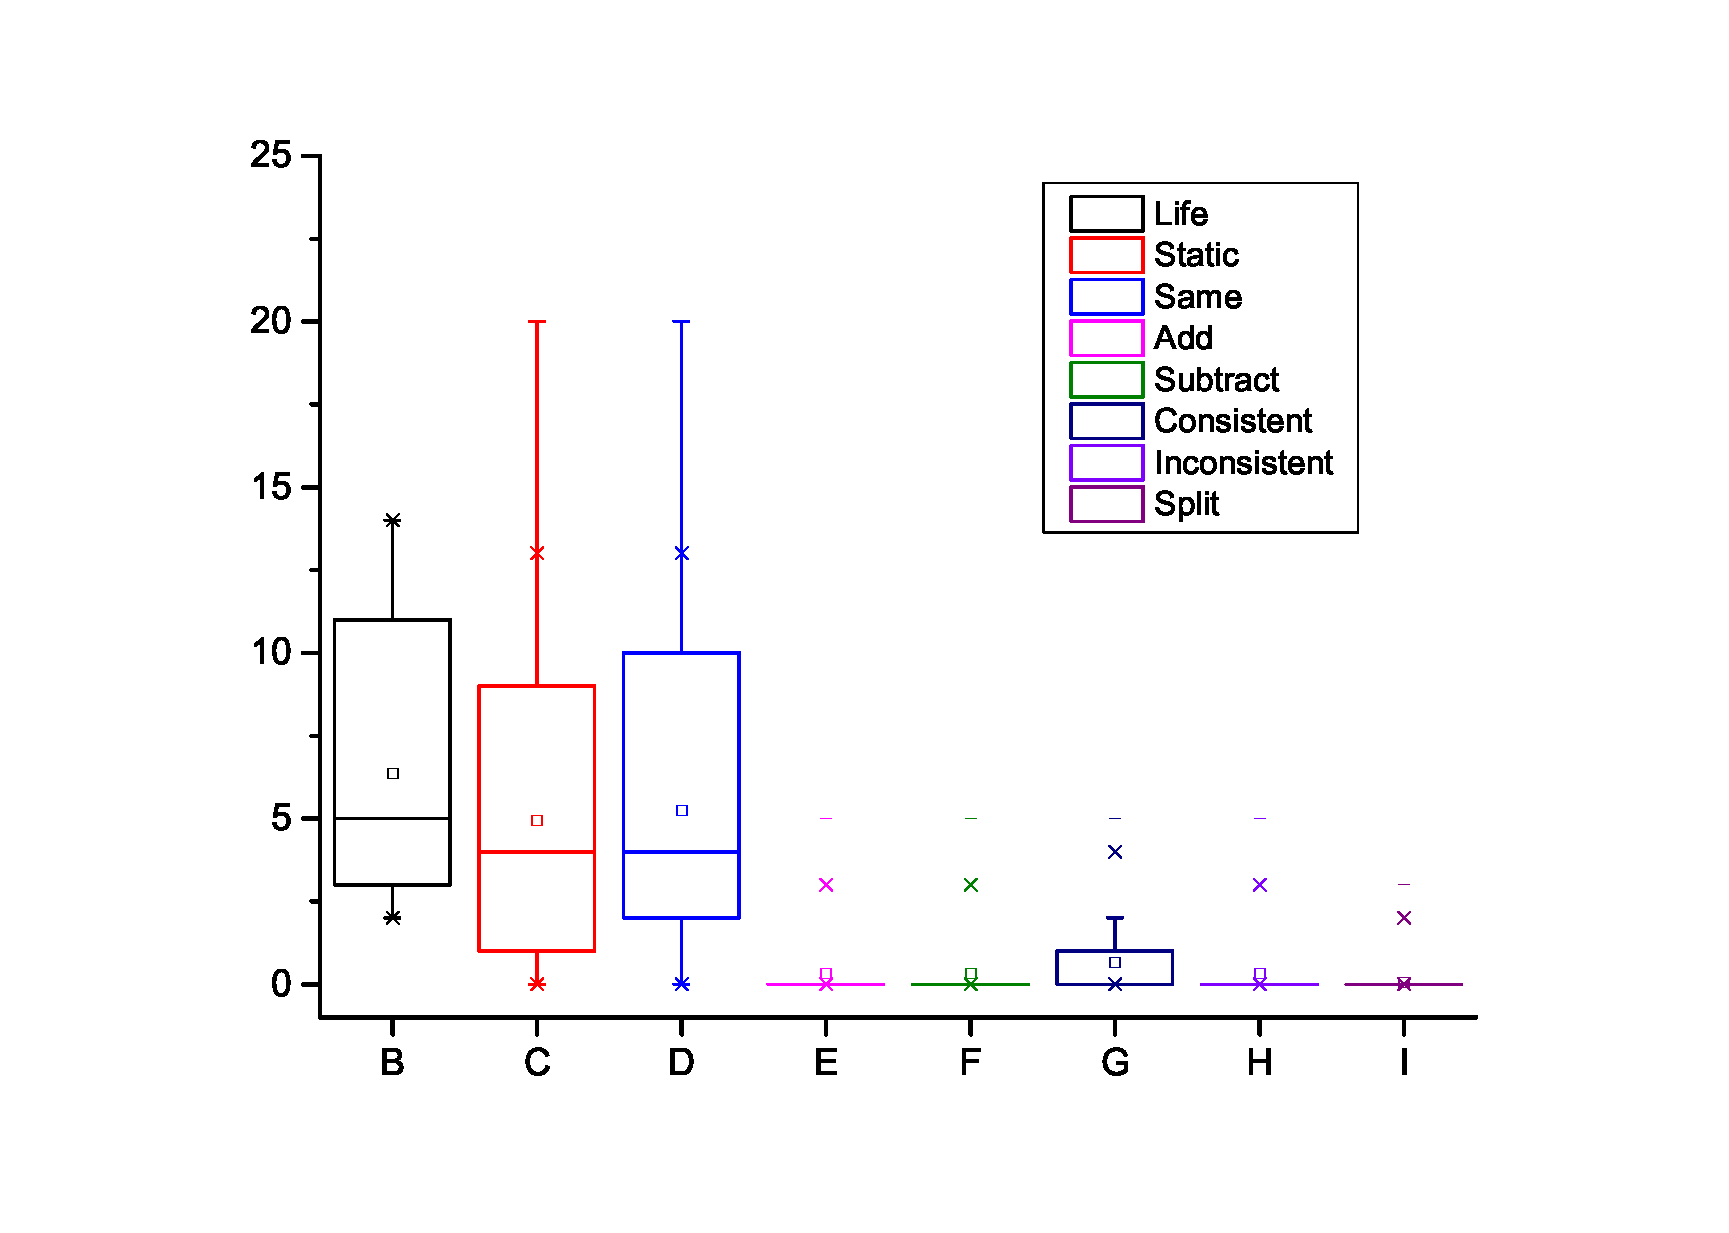
\includegraphics[width=3.3in]{Fig3a.eps} }
    \end{subfigure}
    \begin{subfigure}[jEdit]
    { {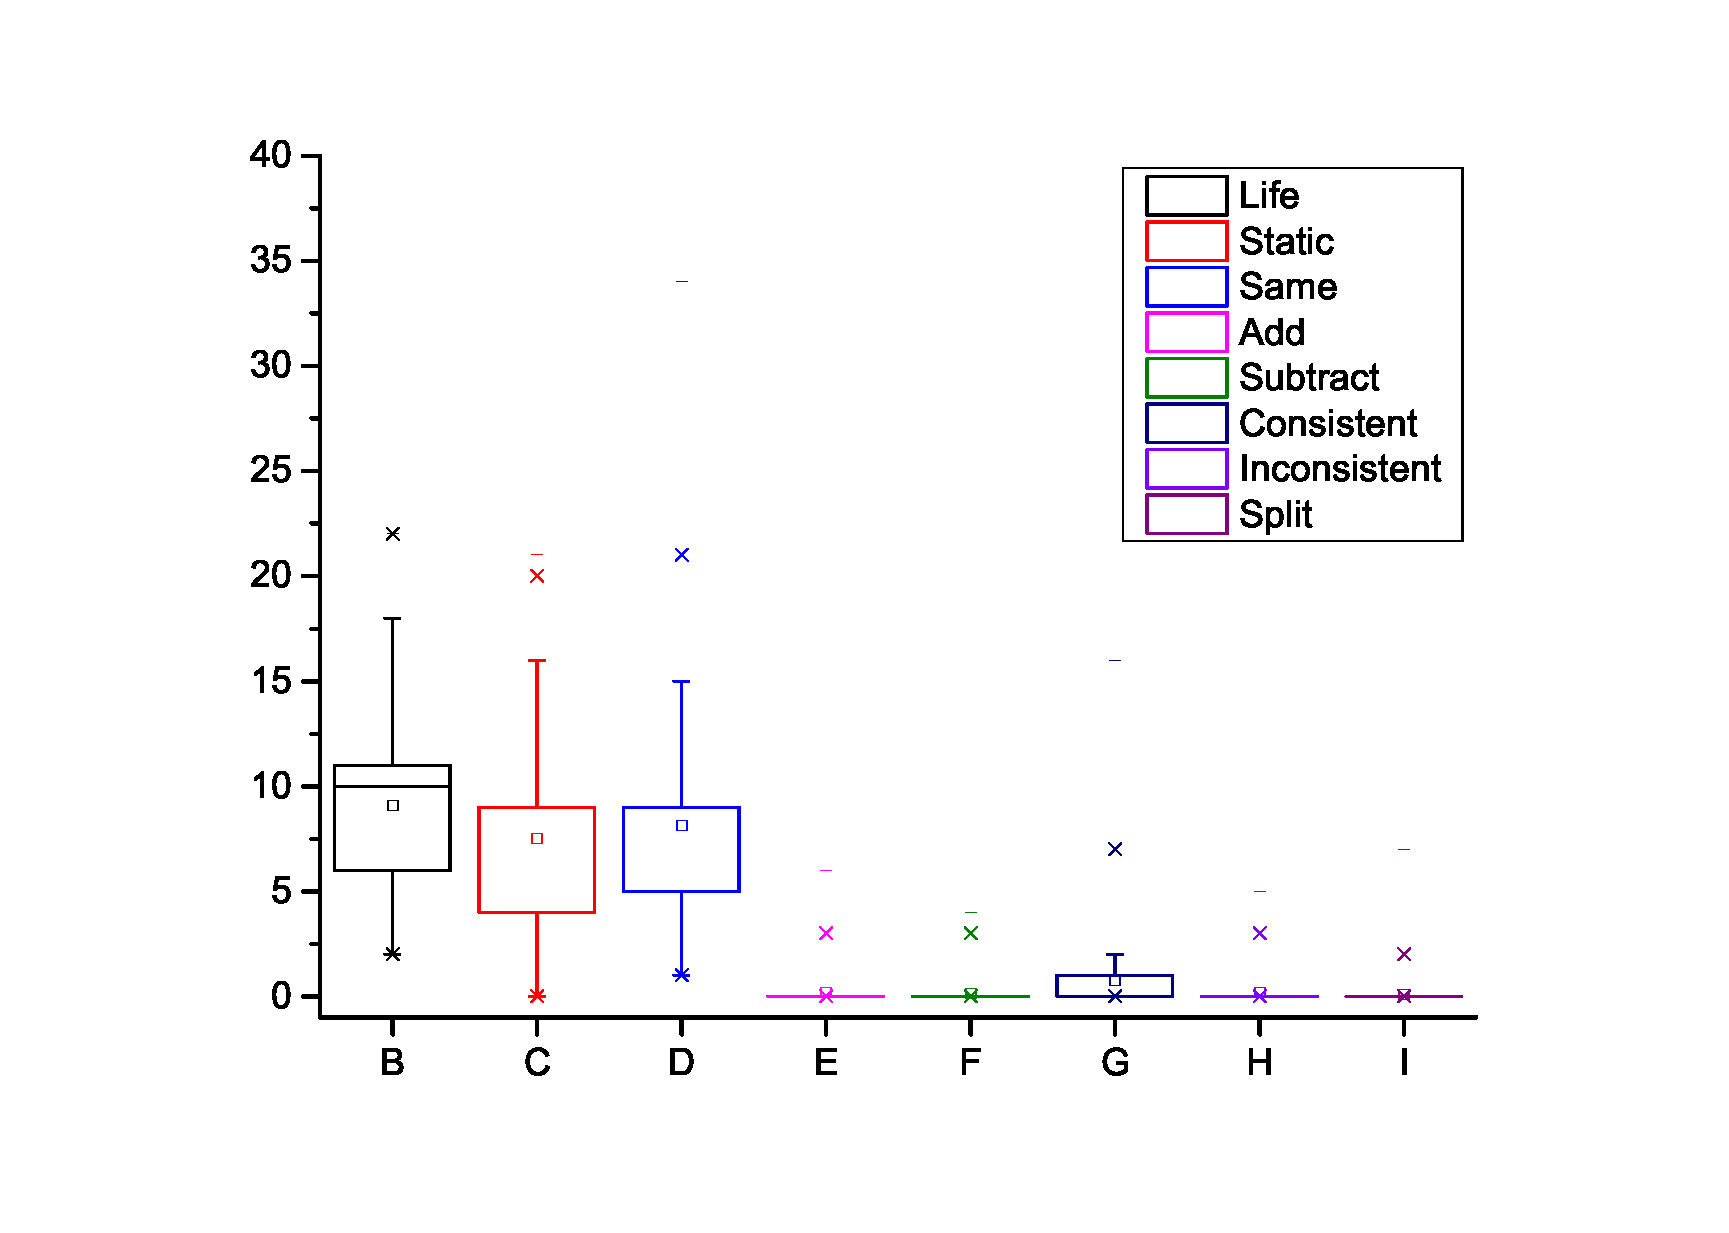
\includegraphics[width=3.3in]{Fig3b.eps} } }
    \end{subfigure}
    \centerline{\footnotesize\begin{tabular}{c} Fig.\ 3.\ Clone Genealogy Statistics Results
\end{tabular}}
\end{figure*}

Tables 8 and 9 depict the results of clone group clustering. Here, Cluster 1 has the largest number of clone groups (71\% in {\em ArgoUML}, 79\% in {\em jEdit}), and these clone groups are relatively stable (have stable clone pattern, do not have dynamic clone pattern), and have relatively longer lives. Therefore, {\em most of clone groups are very stable, which also have a relatively longer life (about 5 versions both in the two software)}. Most of the {\em inconsistent change pattern} appear in Cluster 0, which take up only a small percentage (4\% in {\em ArgoUML}, only 1\% in {\em jEdit}). Therefore, {\em inconsistent change does not frequently occur in clone group}. Meanwhile, {\em consistent change pattern} occurs only in Cluster 2, which also has a relatively longer life --- but shorter than Cluster 0. Both Cluster 0\&2 are dynamic clone groups because they both have the dynamic clone pattern. We conclude that, {\em dynamic clone pattern occurs in longer life clone group, and their number is very small}.  

If we check the absolute number of groups in Cluster 0\&2, we see that the number of clone group having consistent changes (Cluster 2) is bigger than those having inconsistent changes (Cluster 0).  This means {\em consistent change is much easily occurring than inconsistent change}. Thus, we suggest that: {\em Developers should consider the possibility of performing consistent change when they detect that a clone fragment has undergone some change}.  

Cluster 3 shows that there is quite a proportion of clone groups having extremely short life (which just appear in systems), which have no clone pattern. This means that {\em we need not consider the effect of changes in clone group at the initial version of clone group creation}.   

In summary, clone groups are generally very stable throughout evolution. Dynamic clone pattern may happen after the clone groups have been in existence for a while, but only for a small proportion of them. When developers change a particular clone fragment, it is advisable for them to also consider the change in the context of clone group and determine if consistent change need to be made across the entire group.

\leftline{{\bf5.3 \ Clone Genealogy Experiment}}

In studying the characteristics of clone genealogy, which offers a global perspective, we first compute the number of clone pattern occurring in its entire life for each of clone genealogies, and then perform clustering on these clone genealogies using their metrics. 

We first compute the statistics for each of the metrics (including genealogy life and clone patterns) in all the clone genealogies. The results are plotted in Fig.3 using ``Box-and-Whisker'' diagrams.  The first (extreme left) box shows the statistics about genealogy lives. For the rest of the boxes in the plot, each of them represents the statistics for each clone pattern. 

{
\begin{table*}[!htb]
\tabcolsep=2.5pt 
\scriptsize
\begin{center}
\begin{tabular}{|c|c|c|c|c|c|c|c|c|c|c|}
\multicolumn{11}{c}{\bf Table 10.\  Clone Genealogy Clustering Results of ArgoUML }\\ \hline
&Death&&Genealogy Life&	Static&	Same&	Add	&Subtract&	Consistent&	Inconsistent&	Split\\ \hline
Cluster0&\multirow{3}{*}{5}&Mean	&11.85366	&9.79268	&10.45122	&2.23171&	2.23171&	3.06098&	2.29268&	0.39024\\ \cline{3-11}
82&&Standard Deviation	&1.81979	&2.98861&	3.04758&	1.04585&	1.08068	&0.85125&1.07138&	0.84263\\ \cline{3-11}
(8\%)&&Median	&11&	10&	10&	2&	2&	3&	2	&0\\ \hline
Cluster1&\multirow{3}{*}{39}&Mean	&10.19221	&8.83117	&9.0961	&0.17143	&0.12208	&0.44416	&0.12208	&0.00519\\ \cline{3-11}
385&&Standard Deviation&	1.67998	&1.67552	&1.70282	&0.39754&	0.3278	&0.64761&	0.3278	&0.10193\\ \cline{3-11}
(37\%)&&Median	&11	&9	&10	&0&	0&	0&	0	&0\\ \hline
Cluster2&\multirow{3}{*}{188}&Mean	&3.29412	&1.2549	&2	&0.47059	&0.46078	&1.2598	&0.46078	&0.0098\\ \cline{3-11}
204&&Standard Deviation	&1.22847	&1.35506	&1.32427	&0.63875	&0.63822	&0.43961	&0.63822	&0.14003\\ \cline{3-11}
(20\%)&&Median	&3&	1&	2&	0&	0&	1&	0&	0\\ \hline
Cluster3&\multirow{3}{*}{348}&Mean	&2.79452	&1.79452	&1.79452	&0	&0	&0	&0	&0\\ \cline{3-11}
365&&Standard Deviation	&1.0813	&1.0813	&1.0813	&0	&0	&0	&0	&0\\ \cline{3-11}
(35\%)&&Median	&3	&2	&2	&0	&0	&0&	0&	0\\ \hline
All&\multirow{3}{*}{579}&Mean	&6.35907	&4.93629	&5.23359	&0.33301	&0.31274	&0.65541	&0.31757	&0.03475\\ \cline{3-11}
1036&&Standard Deviation	&4.02533	&4.0219	&4.06154	&0.74995	&0.74514	&0.97405	&0.75663	&0.27231\\ \cline{3-11}
(100\%)&&Median&	5&	4&	4&	0&	0&	0&	0&	0\\ \hline
\end{tabular}
\end{center}
\end{table*}
}
{
\begin{table*}[!htb]
\tabcolsep=2.5pt 
\scriptsize
\begin{center}
\begin{tabular}{|c|c|c|c|c|c|c|c|c|c|c|}
\multicolumn{11}{c}{\bf Table 11.\  Clone Genealogy Clustering Results of jEdit }\\ \hline
&Death&&Genealogy Life&	Static&	Same&	Add	&Subtract&	Consistent&	Inconsistent&	Split\\ \hline
Cluster0&\multirow{3}{*}{3}&Mean	&19	&15.8	&19.2	&3	&2.3&	6	&2.7&	1.1\\ \cline{3-11}
10&&Standard Deviation	&4.83046	&4.56557&	6.42564	&1.33333&	0.94868&	4.57044&	1.41814	&2.23358\\ \cline{3-11}
(4\%)&&Median	&22&	17&	19&	3&	2	&4.5	&2.5&	0\\ \hline
Cluster1&\multirow{3}{*}{35}&Mean	&10.95205&	9.44521&	9.93836&	0.07534	&0.07534	&0.58904&	0.08219&	0.0411\\ \cline{3-11}
146&&Standard Deviation&2.35572	&2.16566&2.35832	&0.26485	&0.31262&	1.07428&	0.34254&	0.28471\\ \cline{3-11}
(62\%)&&Median&	10&	9&	9	&0&	0	&0	&0&	0\\ \hline
Cluster2&\multirow{3}{*}{24}&Mean	&6.57143&	4.75&	5.60714&	0.07143&	0.07143&	0.85714&	0.07143&	0.07143\\ \cline{3-11}
28&&Standard Deviation	&1.16837&	1.14261	&1.22744	&0.26227&0.26227	&0.97046	&0.26227	&0.37796\\ \cline{3-11}
(12\%)&&Median	&7	&5	&6&	0	&0	&1&	0&	0\\ \hline
Cluster3&\multirow{3}{*}{48}&Mean	&3.33962&	2.13208&	2.30189&	0.03774&	0	&0.20755&	0	&0\\ \cline{3-11}
53&&Standard Deviation&	0.73231	&0.92065	&0.72284&	0.19238&	0&	0.45398	&0	&0\\ \cline{3-11}
(22\%)&&Median	&3&	2&	2	&0&	0&	0	&0&	0\\ \hline
All&\multirow{3}{*}{110}&Mean	&9.07173	&7.52321&	8.1097	&0.18987&	0.1519&	0.76371	&0.173&	0.08017\\ \cline{3-11}
237&&Standard Deviation	&4.36559&	4.07926	&4.56922	&0.6903&	0.55438&	1.70588	&0.66354	&0.55033\\ \cline{3-11}
(100\%)&&Median	&10	&9	&9	&0	&0	&0	&0	&0\\ \hline
\end{tabular}
\end{center}
\end{table*}
}

We can see that clone genealogy exist in the systems for a reasonably long period of time (i.e.  {\em mean value of life} is 5 versions for {\em ArgoUML} within the entire 14 versions, and 10 versions for {\em jEdit} with the entire 22 versions), and only a small part of clone genealogy exists for extremely short (less than 3 versions) or extremely long (more than 10 versions) life. We also see that the number of {\em stable clone pattern} is much higher than the number of {\em dynamic clone pattern}. For {\em dynamic clone pattern}, their numbers are extremely few, expect for {\em consistent change pattern}. {\em It means that clone genealogy is very stable during the life of clone evolution.} Specially, the number of ``consistent change'' outnumbers that of ``inconsistent change''. This implies that {\em it is worth paying attention to determine if a clone change should be propagated to other clones in the same clone group}. 

We use X-means clustering to mine more information from clone genealogy between the {\em life} and {\em clone patterns}. In Tables 10 and 11, we define a special variable called {\em Death} which reports the number of clone genealogies which have ended their lives before reaching the last version collected in the experiment. By knowing that a genealogy contributes to a count in {\em Death}, we know that the data we obtained in the experiment for clone genealogy is ``complete''; the genealogy does not get terminated prematurely by our selection of software versions.  The second column in these tables thus shows the number of the death clone genealogy. 

According to clustering results, all clone genealogies can be clustered into four clusters, as shown as in the tables. From Fig. 3/Tables 10 \& 11, it is clear that {\em there is a strongly positive correlation between the genealogy life and stable pattern}. We informally define a genealogy to be {\em stable} if it has a high percentage of {\em stable clone pattern}% (which are represented by high numbers of ``static'' and ``same'' metrics)
; otherwise, we say that a genealogy is {\em dynamic}% (that is, it has a relatively large collection of ``add'', ``subtract'', ``consisten'', ``inconsistent'' and ``split'' clone patterns)
. From the tables, we can see that: {\em most of the clone genealogies are stable (Cluster 1,2,3)}. On the other hand, there are much fewer dynamic genealogies (in Cluster 0, having long lives, and most of them are still alive in the systems). It tells us {\em dynamic clone pattern -- especially consistent/inconsistent change -- usually occur in the longer life clone genealogy. Moreover, the number of dynamic genealogy is small}. This suggests that developers should take some measures on {\em dynamic genealogy} because inconsistent change may lead to software defects. For Cluster 3 (both in tables 10,11), the respective clone genealogies have relatively shorter lives, and most of them are already dead. These clone genealogies are extremely stable because the absence of inconsistent pattern. {\em Therefore, it can be concluded that the clones in short life clone genealogies are more stable than the older ones. It can give us a hint that, developers may not need to keep their eyes on newly created (shorter life) clone genealogy. But, they should pay attention to them, when they evolve together with the software.}

In summary, clone genealogies are mostly stable throughout evolution. The shorter-life genealogies are especially stable. {\em Dynamic change pattern} usually occurs among longer-life genealogies, even though the appearance remains sparse. Among them, consistent changes appear more frequently than inconsistent ones. With that, we suggest that developers should pay attention to longer-life clone genealogies, and consider the possibility of allowing consistent change to a clone group when one clone fragment in the group is about to undergo changes.
